\documentclass{acm_proc_article-sp}
\begin{document}
\title{Predicting protein-protein interactions from primary structure using support vector machines}
\numberofauthors{2}
\author{
\alignauthor
Charleston Noble\\
	\affaddr{Northwestern University} \\
	\affaddr{B.A. Mathematics, Bioinformatics, 2012}\\
	\affaddr{charlestonnoble2012@u.northwestern.edu}
% 2nd. author
\alignauthor
Alex Zylman\\
	\affaddr{Northwestern University} \\
	\affaddr{B.S. Computer Engineering, 2012}\\
	\affaddr{azylman@u.northwestern.edu}
}
\maketitle
\begin{abstract}
Predicting whether two given proteins will interact is a central problem in contemporary biological and pharmaceutical research. Here we describe a binary classifier based on support vector learning which accurately predicts protein-protein interaction. In addition to accuracy, our classifier offers plausible extendability to novel, unsynthesized proteins for which we have no information other than their basic amino acid sequences. This no-knowledge requirement would prove invaluable for protein designers, eliminating the intermediate step of synthesizing novel proteins before performing interaction classification.
\end{abstract}

\section{Introduction}
Binding interactions between proteins are essential for the large majority of biological functions. For example, inter- and intra-cellular signals are often transmitted via protein-protein binding, and alteration of these mechanisms is fundamental to many forms of cancer. Even essential processes such as DNA replication and cell recognition rely on interactions between various proteins. Thus predicting interactions between existing and newly synthesized proteins could greatly improve the efficiency of biological and medical research, particularly in the area of novel drug design.

The interaction between proteins is primarily dependent on their tertiary structure. This is the overall three dimensional shape that proteins, or linear chains of amino acids, assume after undergoing a complex, and poorly understood, folding process. It has become widely accepted that the tertiary structure of a protein is directly determined by its primary structure, or the sequence of amino acids which compose it. Thus contemporary techniques for predicting protein-protein interaction bypass the intermediate step of predicting tertiary structure and simply consider the primary structure of the proteins in question \cite{BockNGough}. While protein-protein interaction is not strictly binary (i.e., proteins can interact with varying degrees of strength), for convenience, it is generally treated as such \cite{Yu}.

\section{The Dataset}
The Database of Interacting Proteins, freely available online (http://dip.doe-mbi.ucla.edu), contains over 2664 entries representing pairs of proteins known to mutually bind. It comes in two separate, tab-delimited files: a set of the primary amino acid structures of proteins with an associated DIP ID (30 MB), and a set of proteins pairs that interact (25 MB). The data is labeled by DIP ID for each protein in the pair, whether each of the proteins has any aliases (i.e. a common name), how the interaction was detected, who published the interaction, what publication ID is associated with it, the taxonomic identifiers associated with the proteins, what type of interaction it was, and what the confidence value is. We will only be using the DIP IDs and interaction state to determine positive interactions. 

As for negative interactions, we will use the method of Bock and Gough \cite{BockNGough}. Protein pairs which interact are generally very selective; that is, taking a pair of proteins that interact and changing the positions of only a few amino acids can cause them to lose their positive interaction status. Bearing this in mind, it is plausible that we can choose two proteins from the database which show positive interaction and randomize their respective amino acid sequences, while preserving their amino acid composition and di- and tri-peptide $k$-let frequencies. In so doing, we have created two proteins which likely do not interact, yet are native-like because of conserved higher-order biases. 

This must suffice for numerical experiments, since the task of performing wet experiments to determine every pair that does not, in fact, interact is intractable. By this technique, we do not assume that any pair not found in the database does not interact; we simply make the plausible assumption that altering sequences of interacting proteins causes them to lose their interactivity. Thus we will create random protein pairings to augment our data set such that we have a 1:1 ratio of positive and negative interactions \cite{Fitch, Needleman}.

\section{SVM Learning}
\subsection{Feature vectors}
For each amino acid sequence of a protein-protein pair, individual sequence feature vectors were assembled by ``aggregating" residue descriptors of the constituent amino acids. These included hydrophobicity, hydrophicility, volumes of side chains, polarity, polarizability, solvent-accessible surface area (SASA) and net charge index (NCI). These descriptors were chosen because they, in particular, affect the binding properties of the overall protein \cite{Guo}. The original values of the seven physio-chemical properties for each acid were normalized to zero mean and unit standard deviation, according to Equation (1)
\begin{equation}
P^{'}_{ij}=\frac{P_{i,j}-P_{j}}{SD_{j}}
\end{equation}
where $P_{i,j}$ represents the $j$-th descriptor for the $i$-th amino acid, $P_j$ is the mean of the $j$-th descriptor over the 20 amino acids and $SD_j$ is the corresponding standard deviation.

Now, SVM learning requires a fixed length for feature vectors. Since proteins vary in length, we cannot simply assemble feature vectors consisting of entries for each amino acid, so we ``aggregate" the individual descriptor values to obtain non length-dependent descriptor values for the entire protein chain. For this task, we used the auto-covariance (AC) method of Guo et al. \cite{Guo}. We found the auto-covariance of descriptor values of amino acids a certain distance $lag$ apart on the protein chain. In this way, AC variables can be thought of as the average interaction between amino acid residues, a certain $lag$ apart throughout the sequence. We considered $lag$ values up to a maximum distance $lg$, and so our feature vectors for each individual protein consisted of $7 \times lg $ entries, that is, $lg$ separate AC values for each of the seven descriptors. The AC variables are calculated according to Equation (2),
\begin{eqnarray}\nonumber
AC_{lag,j}=\frac{1}{n-lag}\sum_{i=1}^{n-lag} \left( X_{i,j}-\frac{1}{n}\sum_{i=1}^{n}X_{i,j}\right)\\
\times \left( X_{(i+lag),j}-\frac{1}{n}\sum_{i=1}^{n}X_{i,j}\right)
\end{eqnarray}
where $j$ represents one descriptor, $i$ the position in the sequence $X$, $n$ the length of the sequence $X$ and $lag$ the value of the lag. Once feature vectors were assembled for individual proteins, protein-pairs were represented by concatenating the individual protein vectors. I.e., each protein's feature vector had length $lg\times 7$, so a protein-pair's feature vector had length $2\times lg\times 7$.

\subsection{Training and Testing}
Negative interactions were generated using Shufflet, a bioinformatics application developed by Eivind Coward (Univ. of Bergen), while classification models (and classification predictions) were calculated using a support-vector implementation called SVM light \cite{Joachims}. The final size of the dataset was 134,552 protein-protein pairs; half of these were negative interactions while the other half were positive. An approximately 1:1 ratio was used for training and testing sets.

\section{Results}
We achieved a 72.56\% accuracy rate over the entire dataset using a linear kernel and the full set of features. This compares favorably to the roughly 80\% accuracy of leading research into this problem. From there, we sought to find out which amino acid descriptors had the largest effect in determining the accuracy of our classifier. Initially, we ran our classifier seven times, each time removing precisely one descriptor. Our mean accuracy over these seven classifications was 72.07\% (with a standard deviation of 0.32\%), only slightly less than our accuracy when using all seven descriptors. Of these removals, the removal of SASA had the largest effect, dropping our accuracy to 71.67\%, while the removal of polaizability had the least effect, only dropping our accuracy to 72.46\%. Interestingly, this showed that the addition of a seventh descriptor provided almost no additional accuracy improvement.

From here we explored how the number of descriptors used affects accuracy (Figure 1). Using only one descriptor, the mean accuracy of the classifier dropped to about 60\%, only slightly better than chance. With the addition of one more descriptor, however, our accuracy improved to nearly 70\%. Including additional features after the second yielded minimal accuracy gains, and a remarkably high accuracy can be achieved using only two descriptors. The best combination of descriptors was polarity/SASA, which yielded 70\% accuracy with a linear kernel.

We then switched to a radial basis function kernel, and accuracy improved dramatically. Using polarity as the \emph{only} descriptor, the accuracy of the classifier was 71.4\%, nearly as high as our accuracy using all seven descriptors and a linear kernel. We speculate that running the classifier over the entire dataset with all seven descriptors will improve our accuracy to be on par with the 80\% accuracy of leading methods.

\begin{figure} 
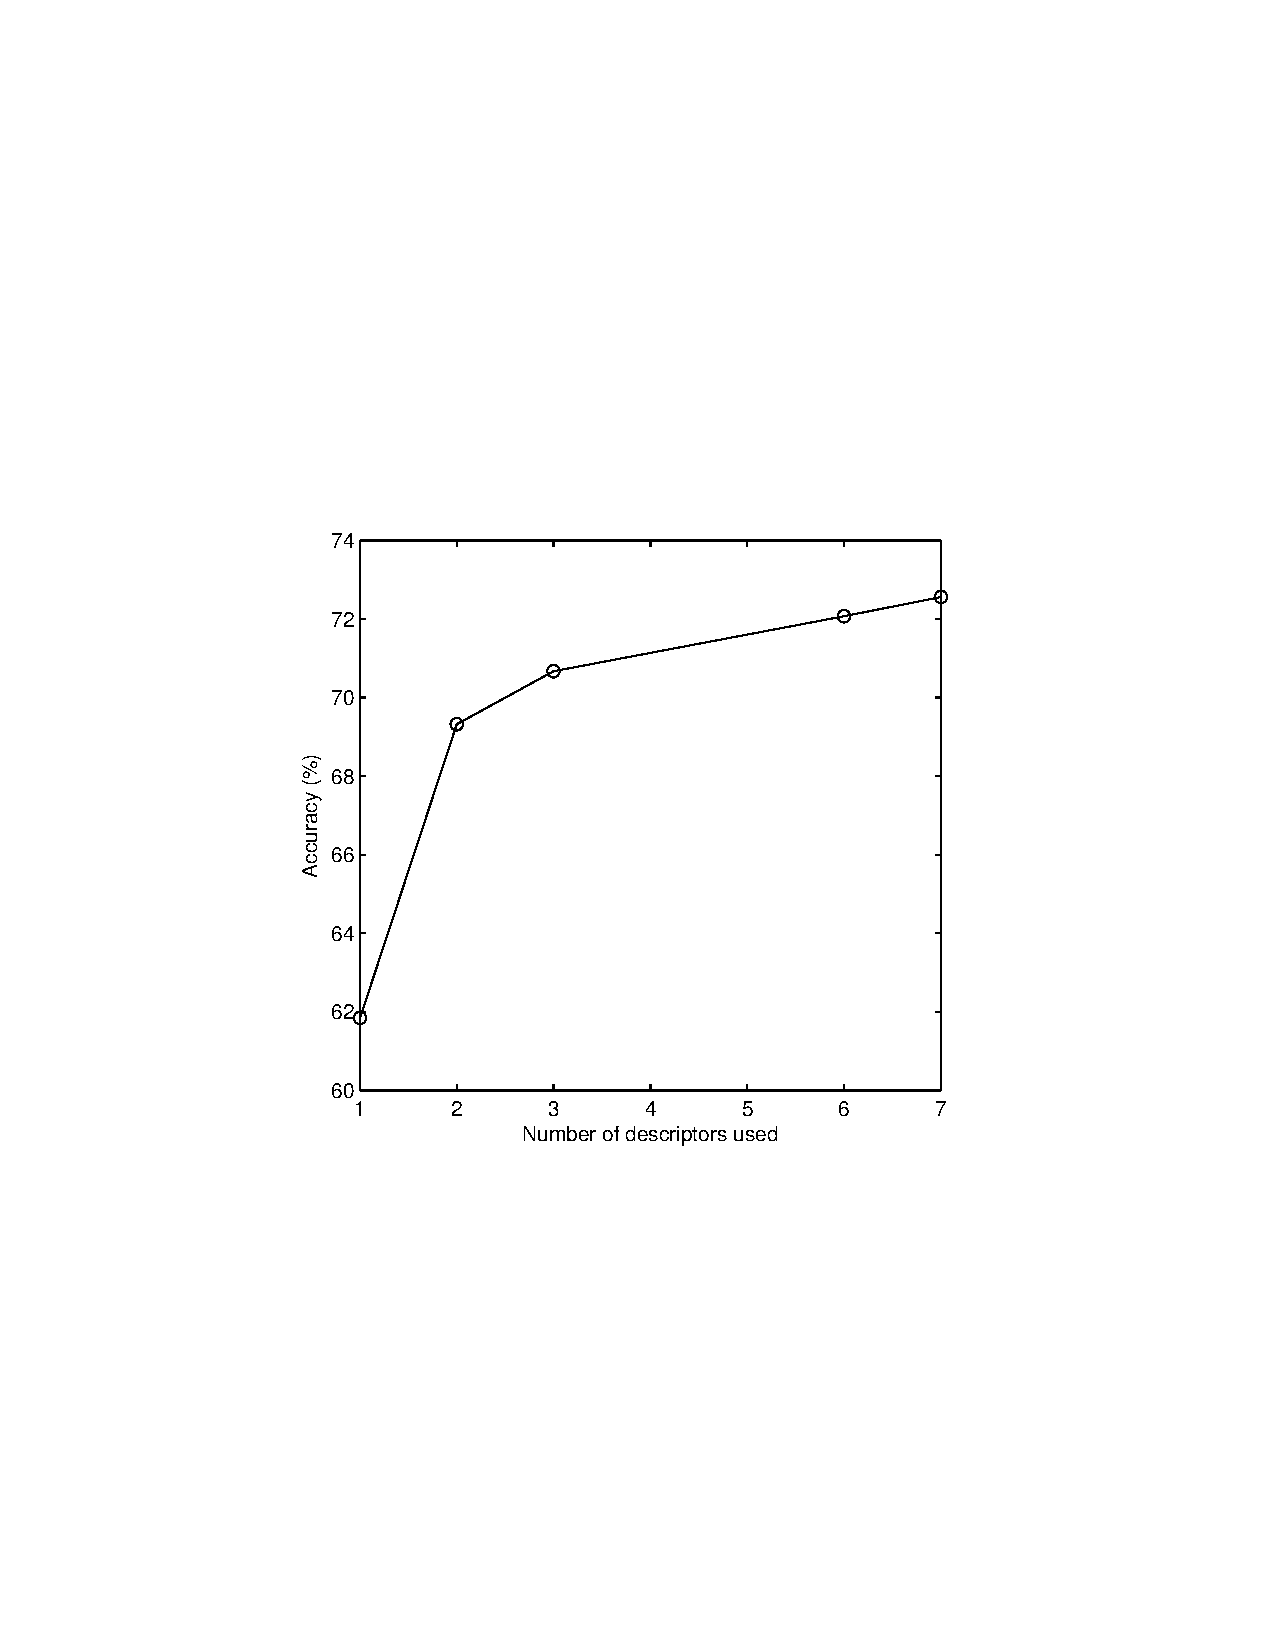
\includegraphics[trim=3cm 9cm 3cm 9cm, width=1\linewidth]{Fig.pdf}
\caption{Accuracy as a function of the number of descriptors used.}
\end{figure}

\bibliographystyle{abbrv}
\bibliography{References}
\balancecolumns
% That's all folks!
\end{document}
